\subsection{Model Environment}

I develop a model of university admissions with students with heterogeneous preference and admission grades and universities with heterogeneous educational quality. First, universities face capacity constraints and must set admission thresholds to manage enrollment. Second, students from different types of schools (public and private) compete for admission through their grades. There are two grading schemes: standardized exams and non-standardized exams. The non-standardized exams are not centrally regulated and grades are assigned based on the student's school, demographic attributes, and subject content. Standardized exams assign grades to students without considering the student's attributes and responding to the student's academic ability. Universities adjust thresholds to match the number of admitted students with their capacity. 

I define how grades are assigned to students differently by exam formats. I define a multivariate function \( F \) that maps the ability and attributes of a student, along with the grading scheme, to a distribution of grades. Formally, let
\[
F: \mathbb{R} \times \mathbb{R}^n \times \{ \text{standardized}, \text{non-standardized} \} \to \mathcal{P}(\{\text{A*}, \text{A}, \text{B}, \ldots\}),
\]
where \( e \in \mathbb{R} \) represents the student's actual ability, \( X \in \mathbb{R}^n \) denotes additional student attributes, and \( \mathcal{P}(\{\text{A*}, \text{A}, \text{B}, \ldots\}) \) represents the set of probability distributions over the ordered grade set.

The grade distribution follows:
\[
F(e, X, Y) \sim \mathcal{M}(\vec{p}(e, X, Y)),
\]
where \( \mathcal{M} \) denotes a multinomial distribution and \( \vec{p}(e, X, Y) \) is a vector of probabilities for each grade, respecting the ordinality of grades from A* to lower grades. The vector \( \vec{p} \) is specified based on whether the grading is standardized or non-standardized:
\[
\vec{p}(e, X, Y) =
\begin{cases}
\vec{p}_s(e), & \text{if } Y = \text{standardized}, \\
\vec{p}_{ns}(e, X), & \text{if } Y = \text{non-standardized}.
\end{cases}
\]
For standardized grading, \( \vec{p}_s(e) \) depends only on the ability of the student \( e \), making the classification process objective. However, under non-standardized grading, \( \vec{p}_{ns}(e, X) \) is influenced by both the ability \( e \) and the additional attributes of the student \( X \), introducing a degree of subjectivity based on contextual factors due to reliance on school context and demographic attributes.


In addition, I define a university capacity function \( G \) that determines enrollment limits. Formally, let
\[
G: \Phi \times \mathbb{R} \to \mathbb{R}^m,
\]
where \( \Phi \subset \mathbb{R}^p \) represents institutional attributes such as funding status and infrastructure, and the second argument represents the overshoot of capacity from the previous year \( \Delta C_{t-1} \). For each university \( i \), I specify:
\[
C_{i,t} = G(\phi_i, \Delta C_{t-1,i}),
\]
where \( \phi_i \in \mathbb{R}^p \) captures the institutional characteristics of the university \( i \) and \( G \) maps institutional characteristics and last year’s capacity overshoot \( \Delta C_{t-1,i}\) 
into the current capacity constraint.

\subsection{Universities and Students}

\subsubsection{Universities}
Consider a market with a finite set of universities $\mathcal{J} = \{1,\ldots,J\}$. Each university $j \in \mathcal{J}$ is characterized by a quality level $Q_j \in \mathcal{R}$, a capacity restriction $C_j \in \mathcal{R}$, and an admission threshold $T_j \in \mathcal{R}$. 

\subsubsection{Students}
% Students
A continuum of students with total mass \(N\) populates the market. Each student \( i \) is characterized by their demographics \( x_i \in \mathcal{R}^n \), attending school type \( s_i \in \{private, public\} \), academic ability score \( e_i^\prime \), and preferences for universities.Note that the observed academic ability score \( e_i^\prime \) is drawn from the grade distribution \(F(e,X,Y)\), where the latent ability \(e\) is transformed by the grading mechanism based on both the student’s attributes \(X\) and the type of exam 
\(Y\).

The student utility for university \( j \) is given by
\[
U_{ij} = e_i^\prime - T_j + \beta Q_j + \epsilon_{ij},
\]
where \( \beta \) represents the preference for university quality and \( \epsilon_{ij} \) is an i.i.d. error term drawn from an extreme value distribution (Type I).

This error structure leads to the multinomial logit model for student choices. The probability that the student \( i \) chooses the university \( j \) is
\[
P_{ij}(T) = \frac{\exp\left(\frac{e_i^\prime - T_j + \beta Q_j}{\mu}\right)}{\sum_{k \in \mathcal{J}} \exp\left(\frac{e_i^\prime - T_k + \beta Q_k}{\mu}\right)},
\]
where \( \mu \) is a scale parameter governing the degree of randomness in the choices.

\subsection{Equilibrium Definition and Characterization}

\subsubsection{Definition}
A market equilibrium consists of admission thresholds $T^* = (T_1^*,\ldots,T_J^*)$ such that:

1. Students make optimal choices given the following utilities: \begin{equation}
       P_{ij}(T^*) = \arg\max_j U_{ij}(T^*)
   \end{equation}

2. Market clearing at each university.: \begin{equation}
       \sum_{i=1}^N P_{ij}(T^*) = C_j \quad \forall j \in \mathcal{J}
   \end{equation}


The equilibrium can be characterized as a fixed point of the system:
\begin{equation}
    \sum_{i=1}^N \frac{\exp((e_i^\prime - T_j + \beta Q_j)/\mu)}{\sum_{k \in \mathcal{J}} \exp((e_i^\prime - T_k + \beta Q_k)/\mu)} = C_j \quad \forall j \in \mathcal{J}
\end{equation}

\begin{figure}
    \centering
    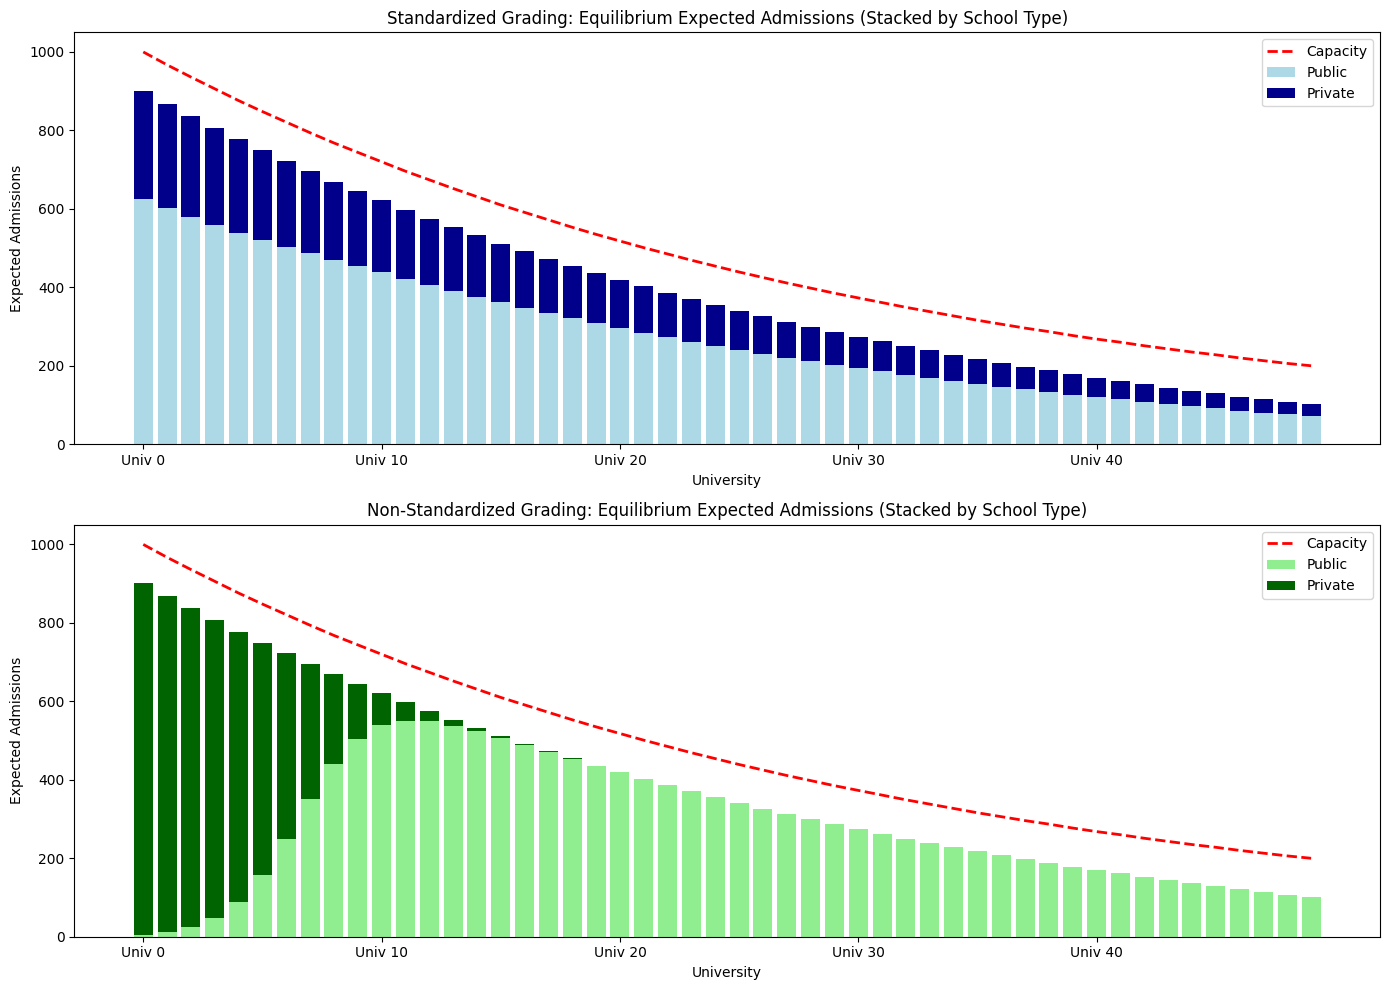
\includegraphics[width=\linewidth]{figures/Empirical_Model/Sorting.png}
    \label{fig:enter-label}
\end{figure}
\subsubsection{Equilibrium Properties}

The equilibrium exhibits several important properties:

1. \textbf{Existence}: An equilibrium exists under mild continuity conditions on student preferences.

2. \textbf{Sorting}: Higher-quality universities set higher equilibrium thresholds: \begin{equation}
       Q_j > Q_k \implies T_j^* > T_k^*
   \end{equation}

3. \textbf{Comparative Statics}: Under non-standardized grading:
   \begin{itemize}
       \item Private school advantage increases with university quality
       \item The gap in admission probabilities between private and public students widens at top universities
   \end{itemize}
